%%%%%%%%%%%%%%%%%%%%%%%%%%%%%%%%%%%%%%%%%%%%%%%%%%%%%%%%%%%%%%%%%%%%%%%%%%
%%%%%                         CHAPITRE 3                            %%%%%%
%%%%%%%%%%%%%%%%%%%%%%%%%%%%%%%%%%%%%%%%%%%%%%%%%%%%%%%%%%%%%%%%%%%%%%%%%%

\lhead[\fancyplain{}{\leftmark}]%Pour les pages paires \bfseries
      {\fancyplain{}{}} %Pour les pages impaires
\chead[\fancyplain{}{}]%
      {\fancyplain{}{}}
\rhead[\fancyplain{}{}]%Pour les pages paires 
      {\fancyplain{}{\rightmark}}%Pour les pages impaires \bfseries
\lfoot[\fancyplain{}{}]%
      {\fancyplain{}{}}
\cfoot[\fancyplain{}{\thepage}]%\bfseries
      {\fancyplain{}{\thepage}} %\bfseries
\rfoot[\fancyplain{}{}]%
     {\fancyplain{}{\scriptsize}}


%%%%%%%%%%%%%%%%%%%%%%%%%%%%%%%%%%%%%%%%%%%%%%%%%%%%%%%%%%%%%%%%%%%%%%%%%%
%%%%%                      Start part here                          %%%%%%
%%%%%%%%%%%%%%%%%%%%%%%%%%%%%%%%%%%%%%%%%%%%%%%%%%%%%%%%%%%%%%%%%%%%%%%%%%

\chapter{Proposed solution: Pose2Sim Python package}
\label{ch:3}

%==============================================================================	Résumé du chapitre

\begin{center}
\rule{0.7\linewidth}{.5pt}
\begin{minipage}{0.7\linewidth}
\smallskip

\textit{We propose the Pose2Sim python package, as an alternative to the more usual marker-based motion capture methods.Pose2Sim stands for "OpenPose to OpenSim", as it uses OpenPose inputs (2D keypoints coordinates obtained from multiple videos) and leads to an OpenSim result (physically consistent full-body 3D joint angles). Code is available at \url{https://github.com/perfanalytics/pose2sim}. \newline \newline
This chapter is adapted from the article published in the Journal of Open Source Software: "Pose2Sim: An Open-source Python Package for multiview markerless kinematics" \cite{Pagnon2022b}.}

%\smallskip
\end{minipage}
\smallskip
\rule{0.7\linewidth}{.5pt}
\end{center}

\minitoc
\newpage


% Sections 
% Intro: motivation, workflow, install, demo
% Method details: Project, 2D kpt detec, calib, track, trig, filt & others, opensim scale & IK

% Mix JOSS & github


\section{Introduction to the workflow}

Although some developments are relevant to both, specifics differ between medicine and the sports field. In this regard and as stated in the \nameref{sec:statement of need}, marker-based methods are not well suited for sports motion analysis \cite{Colyer2018}. In sports, capture should not hinder the movement. Placing markers on the naked body takes time and is cumbersome, therefore markerless approaches are favored. Sports environments are usually much more challenging than lab settings: frequent occlusions, fast and unusual movements, and complex background make it important to resort to using multiple view points, from RGB rather than RGB-D cameras, processed with machine learning methods. Competition conditions are often fast-paced and congested, so a light-weight, fast, and easy to set up system is relevant. However, as coaches and athletes usually need a mere feedback rather than a definitive diagnosis, they don't need as thorough of an accuracy as physicians. Ideally, results should be given in real time, and they should be more visual than graphs of time series. Moreover, 3D kinematics are more relevant than 2D sagittal plane kinematics; and full-body analysis (including upper-limb) is desired.

We propose the Python package Pose2Sim \cite{Pagnon2022b}, which aims to deal with these constraints. It provides a framework for 3D markerless kinematics, as an alternative to the more usual marker-based motion capture methods. Pose2Sim stands for "OpenPose to OpenSim", as it uses OpenPose inputs (2D coordinates obtained from multiple videos) \cite{Cao2019} and leads to an OpenSim result (full-body 3D joint angles) \cite{Delp2007,Seth2018}. Pose2Sim is accessible at \url{https://github.com/perfanalytics/pose2sim}.

\begin{figure}[hbtp]
	\centering
	\def\svgwidth{1\columnwidth}
	\fontsize{10pt}{10pt}\selectfont
	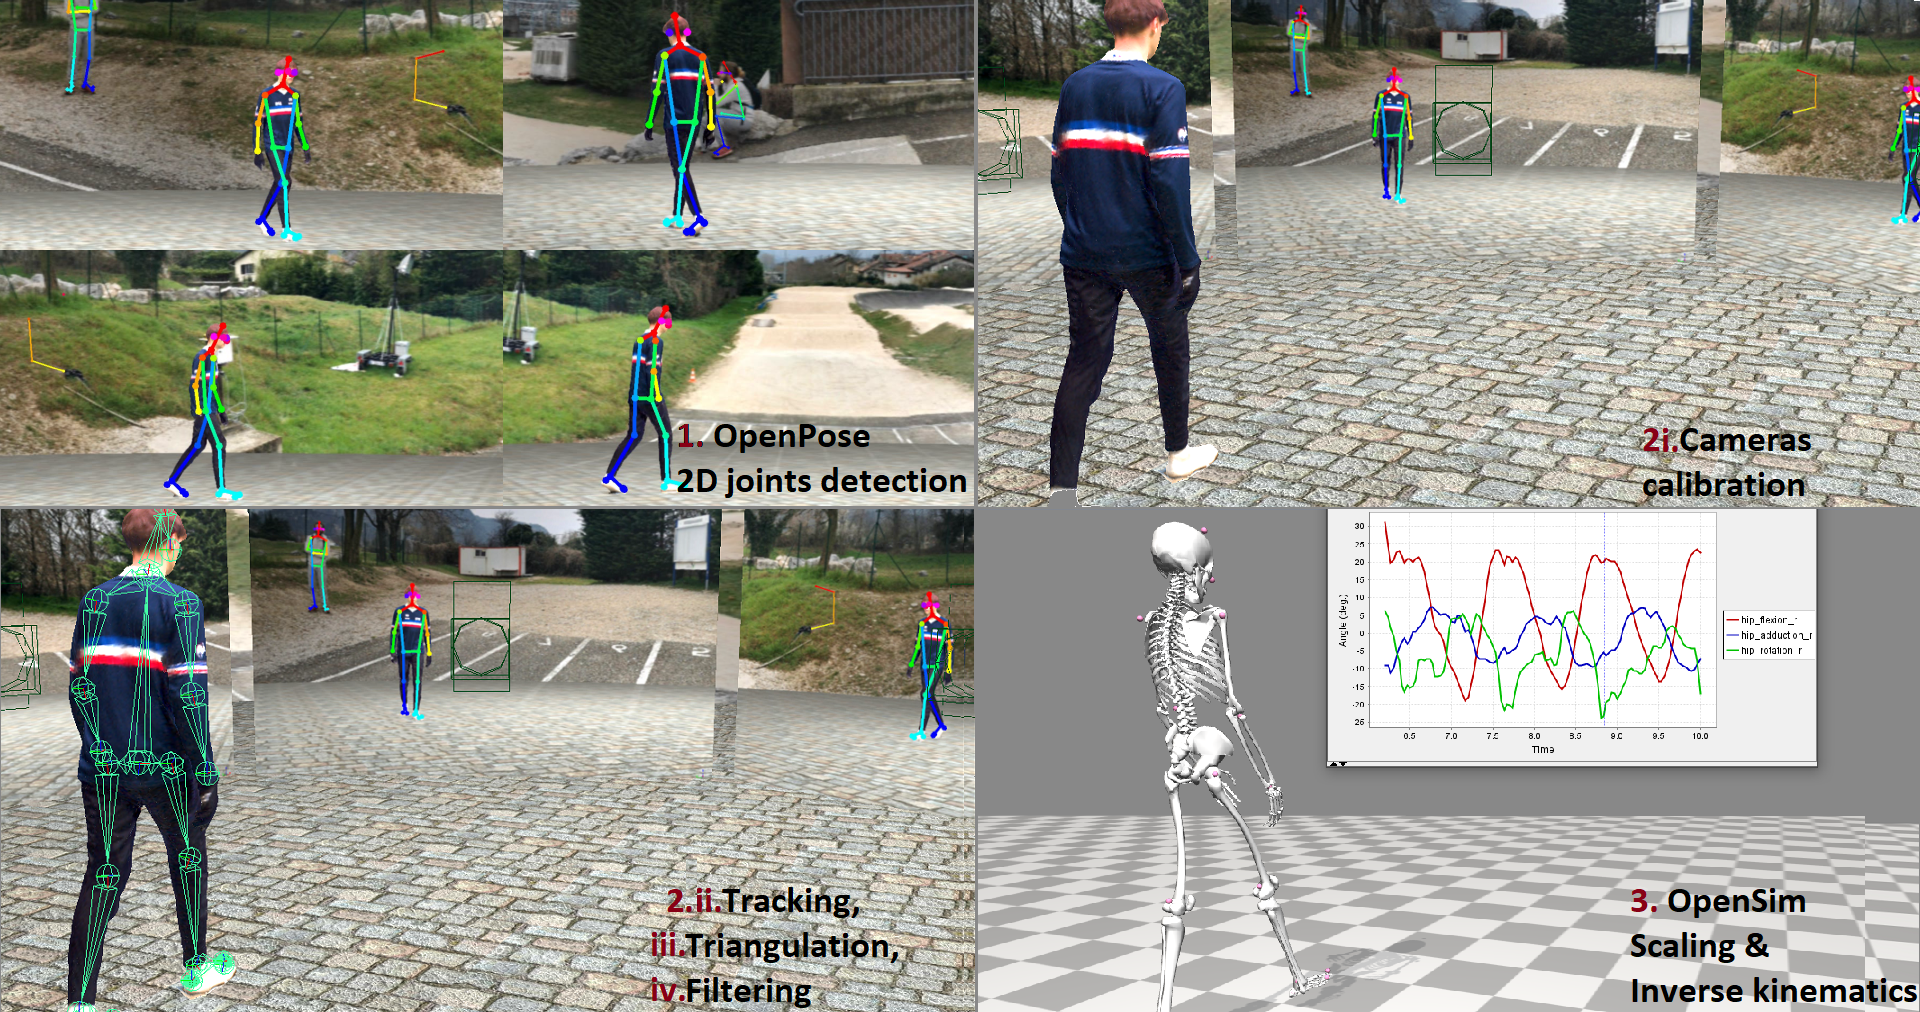
\includegraphics[width=\linewidth]{"../Chap3/Figures/Pipeline.png"}
	\caption{Pose2Sim full pipeline: (1) 2D keypoint detection; (2.1) Camera calibration; \newline(2.1-2.4) Tracking of the person of interest, Triangulating of keypoint coordinates; and Filtering; (3) Constraining the 3D coordinates to an individually scaled, physically consistent OpenSim skeletal model.}
	\label{fig_pipeline}
\end{figure}

\newpage

The repository presents a framework which consists in (Figures~\ref{fig_pipeline}):
\begin{enumerate}[itemsep=0em, topsep=0em, leftmargin=*]
      \item Preliminary 2D joint coordinate detections from multiple videos, e.g. with OpenPose.
      \item Pose2Sim core, including 4 customizable steps:
      \begin{enumerate}[before=\vspace{-0.5\baselineskip}, nosep, label*=\arabic*.]
            \item Camera calibration.
            \item 2D tracking of the person of interest.
            \item 3D keypoint triangulation.
            \item 3D coordinate filtering.
      \end{enumerate}
      \item Scaling a full-body skeleton to each individual subject, and computing inverse kinematics via OpenSim so as to obtain 3D joint angles.
\end{enumerate}

\vskip 1em

Each task is easily customizable, and requires only moderate Python skills. The whole workflow runs from any video cameras, on any computer, equipped with any operating system (although OpenSim has to be compiled from source on Linux.) Pose2Sim has already been used and tested in a number of situations (walking, running, cycling, dancing, balancing, swimming, boxing), and published in peer-reviewed scientific publications assessing the quality of its code \cite{Pagnon2022c}, its robustness (see Chapter 4 on \nameref{ch:4}) \cite{Pagnon2021} and its accuracy (see Chapter 5 on \nameref{ch:5}) \cite{Pagnon2022a}. Its results for inverse kinematics were deemed good when compared to marker-based ones, with errors generally below 4.0° across several activities, on both lower and on upper limbs. The combination of its ease of use, customizable parameters, and high robustness and accuracy makes it promising, especially for "in-the-wild" sports movement analysis.


\section{Installation and demonstration}

\subsection{Installation}

\begin{enumerate}[itemsep=0em, topsep=0em, leftmargin=*]
      \item Install \textbf{OpenPose} (instructions \href{https://github.com/CMU-Perceptual-Computing-Lab/openpose/blob/master/doc/installation/0_index.md}{here}).\newline
      Windows portable demo is enough.
      \item Install \textbf{OpenSim 4.x} from \href{https://simtk.org/frs/index.php?group_id=91}{there}.\newline
      Tested up to v4.4-beta on Windows. Has to be compiled from source on Linux (see \href{https://simtk-confluence.stanford.edu:8443/display/OpenSim/Linux+Support}{there}.
      \item \textit{Optional:} Install \textbf{Anaconda} or \href{https://docs.conda.io/en/latest/miniconda.html}{Miniconda}.\newline
      Open an Anaconda terminal and create a virtual environment by typing:
      \begin{minted}[frame=single, rulecolor=\color{gray!40}, autogobble]{shell-session}
            conda create -n Pose2Sim python=3.8.8
            conda activate Pose2Sim
      \end{minted}
      \item Install \textbf{Pose2Sim}\newline
      If you don't use Anaconda, type \mintinline{shell-session}{python -V} in terminal to make sure python>=3.6 is installed.
      \begin{itemize}
            \item OPTION 1: \textit{Quick install.} Type in terminal:
            \begin{minted}[frame=single, rulecolor=\color{gray!40}, autogobble]{shell-session}
                  pip install pose2sim
            \end{minted}
            \item OPTION 2: \textit{Build from source.} Open a terminal in the directory of your choice and clone the Pose2Sim repository:
            \begin{minted}[frame=single, rulecolor=\color{gray!40}, autogobble]{shell-session}
                  git clone https://gitlab.inria.fr/perfanalytics/pose2sim.git
                  cd pose2sim
                  pip install .
            \end{minted}
      \end{itemize}
\end{enumerate}


\subsection{Demonstration Part-1: Build 3D TRC file on Python}

This demonstration provides an example experiment of a person balancing on a beam, filmed with 4 calibrated cameras processed with OpenPose.

Open a terminal and check package location with  \mintinline{shell-session}{pip show pose2sim | grep Location}. \newline
Copy this path and go to the Demo folder with  \mintinline{shell-session}{cd <path>\pose2sim\Demo`}. \newline
Type \mintinline{shell-session}{python}, and test the following code (Figures~\ref{fig_pose2sim}):
\begin{minted}[frame=single, rulecolor=\color{gray!40}, autogobble]{python}
      from Pose2Sim import Pose2Sim
      Pose2Sim.calibrateCams()
      Pose2Sim.track2D()
      Pose2Sim.triangulate3D()
      Pose2Sim.filter3D()
\end{minted}

You should obtain a plot of all the 3D coordinates trajectories (Figures~\ref{fig_filterplot}). You can check the logs in \mintinline{shell-session}{Demo\Users\logs.txt}. Results are stored as .trc files in the \mintinline{shell-session}{Demo\pose-3d} directory (Figures~\ref{fig_trc}). Note that when the functions are called without any argument, the Config file is searched in the default \mintinline{shell-session}{Users\Config.toml} location. These parameters can be edited by the user.

\begin{figure}[hbtp]
	\centering
	\def\svgwidth{1\columnwidth}
	\fontsize{10pt}{10pt}\selectfont
	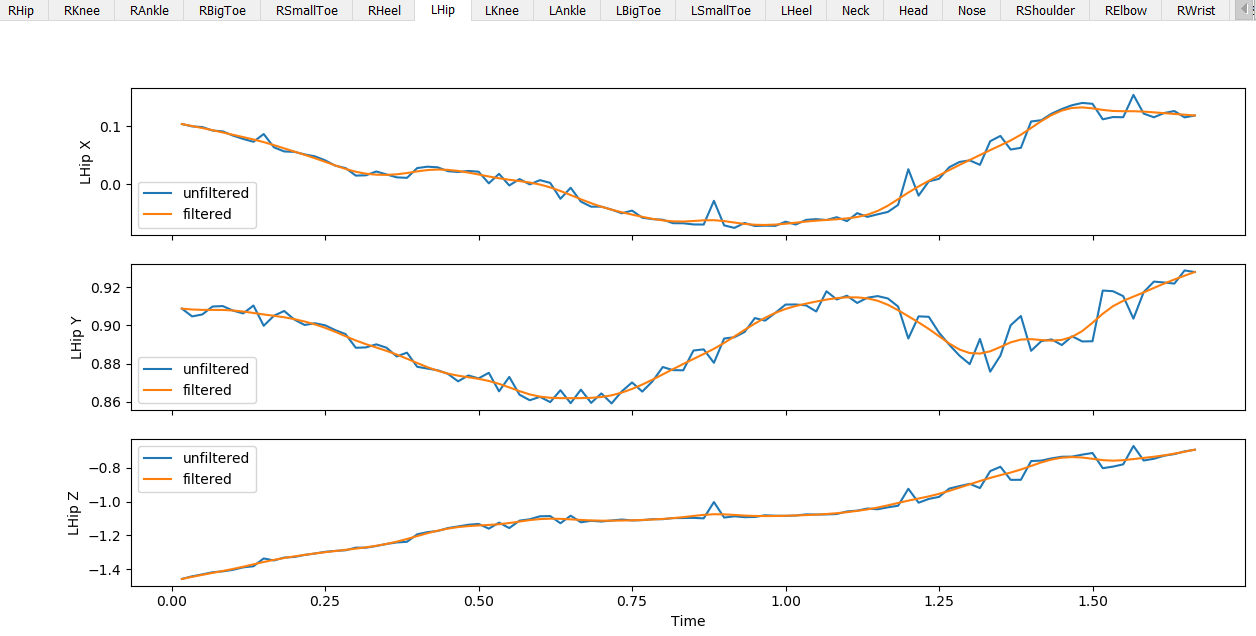
\includegraphics[width=\linewidth]{"../Chap3/Figures/FilterPlot.png"}
	\caption{Filtering results, for each keypoint in a different tab.}
	\label{fig_filterplot}
\end{figure}

\begin{figure}[hbtp]
	\centering
	\def\svgwidth{1\columnwidth}
	\fontsize{10pt}{10pt}\selectfont
	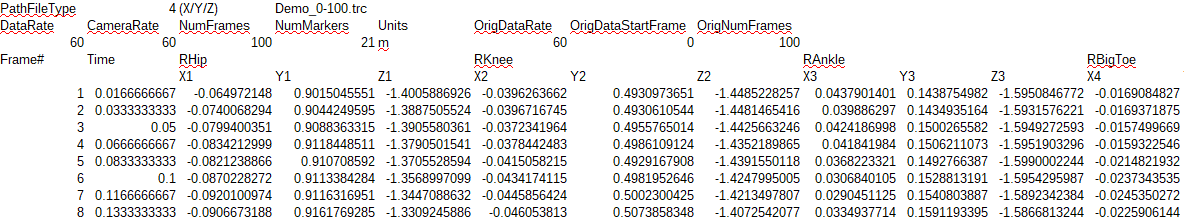
\includegraphics[width=\linewidth]{"../Chap3/Figures/Trc.png"}
	\caption{An example .trc file of triangulated keypoint coordinates, directly usable in OpenSim.}
	\label{fig_trc}
\end{figure}

\begin{figure}[hbtp]
	\centering
	\begin{subfigure}[b]{1\textwidth}
		\centering
		\def\svgwidth{\columnwidth}
		\fontsize{10pt}{10pt}\selectfont
		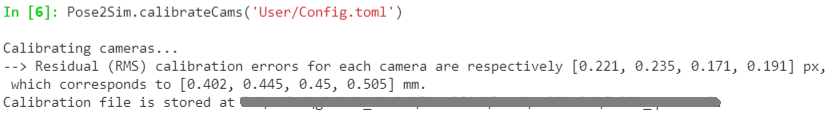
\includegraphics[width=\linewidth]{"../Chap3/Figures/Calib2D.png"}
            \caption{Calibration can either be done from a checkerboard, or by simply converting a Qualisys calibration file. Calibration errors are computed and provided.\newline}
      \end{subfigure}
	\qquad
	\begin{subfigure}[b]{1\textwidth}
		\centering
		\def\svgwidth{\columnwidth}
		\fontsize{10pt}{10pt}\selectfont
		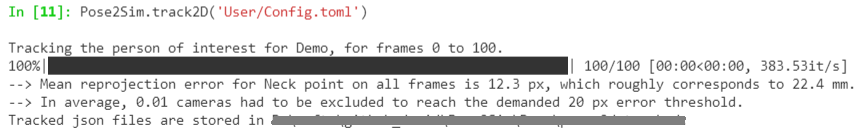
\includegraphics[width=\linewidth]{"../Chap3/Figures/Track2D.png"}
            \caption{If several persons are detected in the scene, a tracking step can be carried out in order to make sure that the right person from each camera will be triangulated.}
      \end{subfigure}
      \begin{subfigure}[b]{1\textwidth}
		\centering
		\def\svgwidth{1\columnwidth}
		\fontsize{10pt}{10pt}\selectfont
		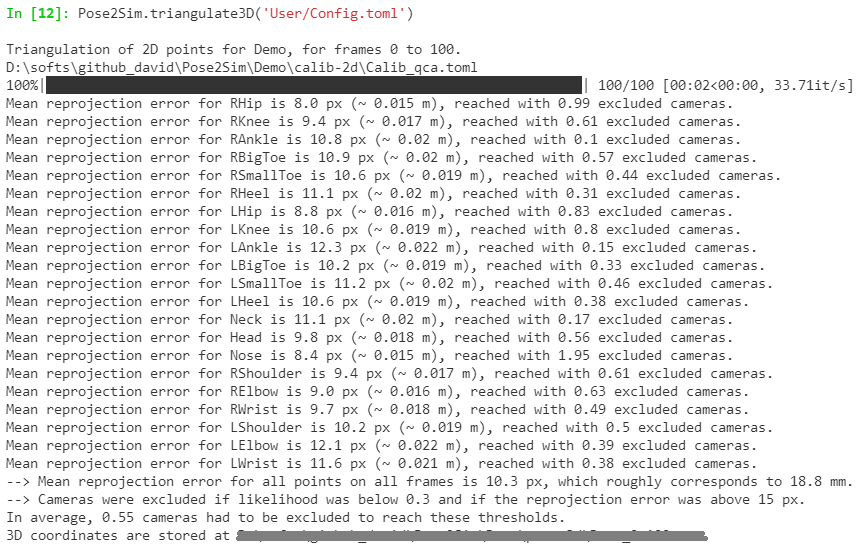
\includegraphics[width=\linewidth]{"../Chap3/Figures/Triangulate3D.png"}
            \caption{The triangulation is weighted by the OpenPose likelihood, and constrained by some thresholds defined in the Config.toml file. If these constraints are not met, e.g., if the reprojection error is too large or if the likelihood of a keypoint is too low, one or several cameras are excluded. The mean reprojection error and the number of cameras that have been excluded to meet the constraints is printed, for each keypoints.}
      \end{subfigure}
      \begin{subfigure}[b]{1\textwidth}
		\centering
		\def\svgwidth{1\columnwidth}
		\fontsize{10pt}{10pt}\selectfont
		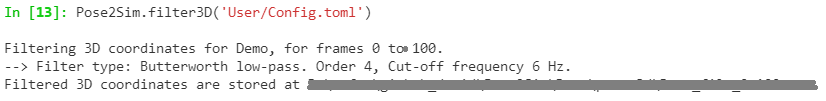
\includegraphics[width=\linewidth]{"../Chap3/Figures/Filter3D.png"}
            \caption{Triangulated data can be filtered, either with a low-pass Butterworth filter or with other types, and parameters can be adjusted.}
      \end{subfigure}
	\caption{First steps of Pose2Sim pipeline in Python. Calibration can either be done from a checkerboard, or by simply converting a Qualisys calibration file. Note that the functions can be used without any arguments if the Config.toml file is left in the default location.}
	\label{fig_pose2sim}
\end{figure}


\FloatBarrier
\subsection{Demonstration Part-2: Obtain 3D joint angles with OpenSim}
In the same vein as we would do with marker-based kinematics, the model first needs to be scaled to each individual, and then inverse kinematics can be performed (Figures~\ref{fig_opensimdemo}).

\textbf{Scaling:}
\begin{enumerate}[itemsep=0em, topsep=0em, leftmargin=*]
      \item Open OpenSim.
      \item Open the provided \mintinline{shell-session}{Model_Pose2Sim_Body25b.osim} model from \mintinline{shell-session}{pose2sim/Demo/opensim}. (File $\mapsto$ Open Model)
      \item Load the provided \mintinline{shell-session}{Scaling_Setup_Pose2Sim_Body25b.xml} scaling file from \mintinline{shell-session}{pose2sim/Demo/opensim}. (Tools $\mapsto$ Scale model $\mapsto$ Load)
      \item Run. You should see your skeletal model take the static pose.
\end{enumerate}

\textbf{Inverse kinematics}
\begin{enumerate}[itemsep=0em, topsep=0em, leftmargin=*]
    \item Load the provided \mintinline{shell-session}{IK_Setup_Pose2Sim_Body25b.xml} scaling file from \mintinline{shell-session}{pose2sim/Demo/opensim}. (Tools $\mapsto$ Inverse kinematics $\mapsto$ Load)
    \item Run. You should see your skeletal model move in the Vizualizer window.
\end{enumerate}

\begin{figure}[hbtp]
	\centering
	\def\svgwidth{1\columnwidth}
	\fontsize{10pt}{10pt}\selectfont
	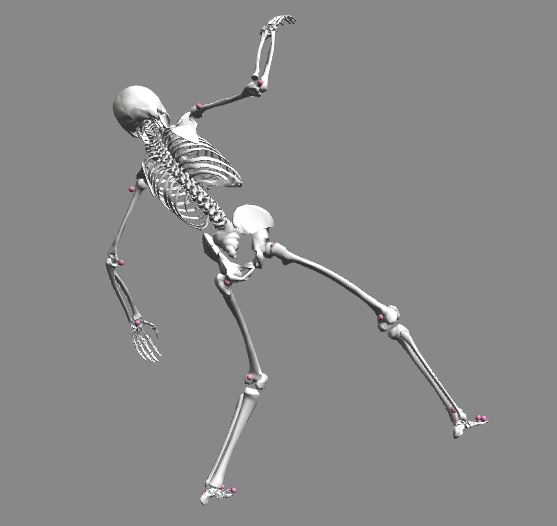
\includegraphics[width=\linewidth]{"../Chap3/Figures/OpenSimDemo.JPG"}
	\caption{At the end of the demonstration, you should have a skeleton balancing on a beam in OpenSim.}
	\label{fig_opensimdemo}
\end{figure}


\section{Method details}

\subsection{Project}
Pose2Sim is meant to be as fully and easily configurable as possible, by editing the \mintinline{shell-session}{User/Config.toml} file. First of all, the user can specify the project path and folder names, the video frame rate, and the range of analyzed frames. Optional tools are also provided for extending its usage (Figures~\ref{fig_opensimutilities}). More practical information can be found on the GitHub repository. 

\begin{figure}[hbtp]
	\centering
	\def\svgwidth{1\columnwidth}
	\fontsize{10pt}{10pt}\selectfont
	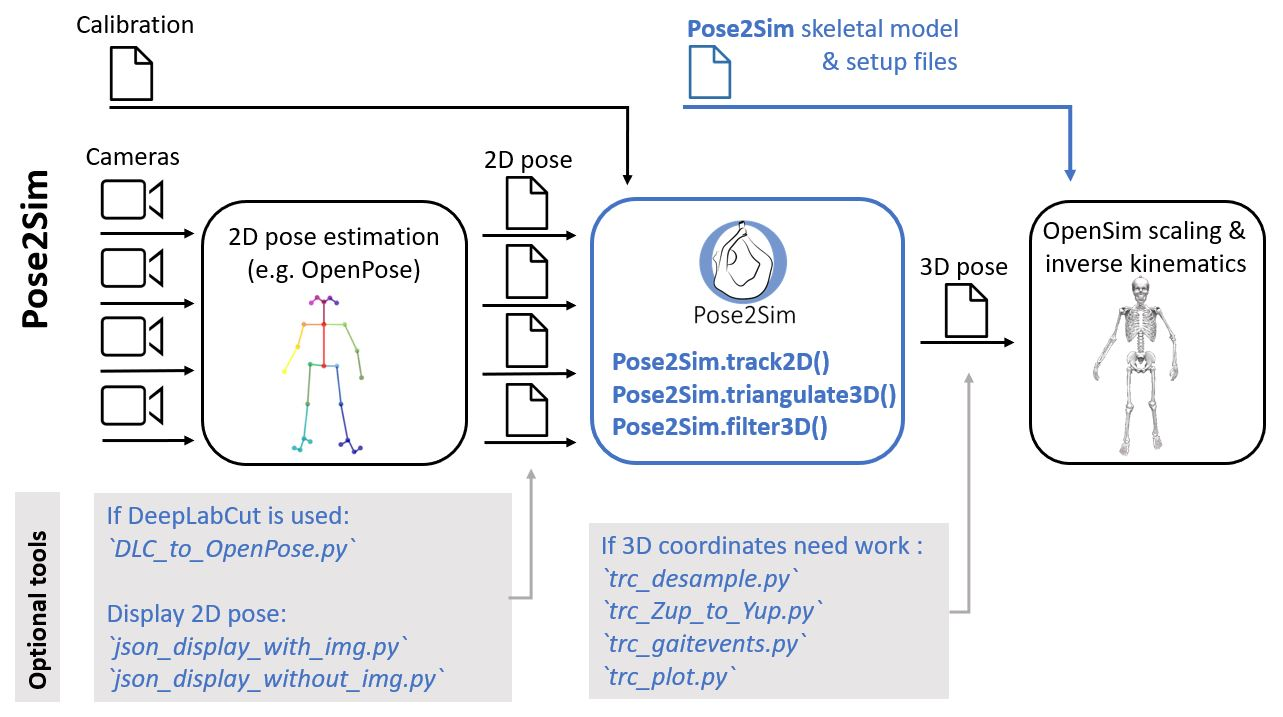
\includegraphics[width=\linewidth]{"../Chap3/Figures/Pose2Sim_utilities.jpg"}
	\caption{The Pose2Sim workflow, along with some optional utilities provided in the package.}
	\label{fig_opensimutilities}
\end{figure}


\subsection{2D keypoint detection}

The interest in deep-learning pose estimation neural networks has been growing fast since 2015 \cite{Zheng2022}, which makes it now possible to collect accurate and reliable 2D landmark positions without the use of physical markers. OpenPose, for example, is a widespread open-source software which provides 2D joint coordinate estimates from videos. As it is the software we have extensively tested, we recommend choosing it.

Feet are usually needed in sports kinematic analysis, and OpenPose is one of the few programs which can detect them. Indeed, it comes with \{body + feet\} models such as body\_25 or body\_25B, as well as with a \{body + feet + hands + face\} one called body\_135 \cite{Hidalgo2019}. The latter two are more accurate than the standard body\_25 one. However, body\_135 requires high computational resources, unlike body\_25B which is as fast as body\_25, and which we have extensively tested \cite{Pagnon2022a}. Hence, we recommend using it. Note that only 21 of the 25 detected keypoints are tracked, since eye and ear keypoints would be redundant in the determination of the head orientation. 

This being said, the user can choose any deep-learning pose estimation network. This choice will affect how keypoint indices will be mapped to model markers in OpenSim, corresponding to anatomical landmarks or joint centers. The OpenPose body\_25, body\_25B, body\_135, COCO, and MPII models are fully supported. The AlphaPose COCO, COCO-WholeBody, and full-body HALPE models are also supported, as well as the full-body but single-person detection BlazePose model. COCO and MPII model are the ones generally used by other networks such as OpenPifPaf \cite{Kreiss2021}, YOLO-pose \cite{Maji2022, Wang2022b}, and others, which means that they are also supported. It is also possible to build custom skeletons in the \mintinline{shell-session}{skeleton.py} file, trained for example with DeepLabCut \cite{Mathis2018, Lauer2022} or SLEAP \cite{Pereira2022}. They will be triangulated, but the user will need to build an OpenSim model and set the keypoints in the right place before being able to perform inverse kinematics.

%%%%%%%%%%%%%%%%%%%%%%%%%%%%%%%%%%%%%%%%%%%%%%%%%%%%%%%%%%%%%%%%%%%
% ATTENTION:                                                      %
% IMPLEMENTER CES MODELES ET LES TESTER AVANT DE PUBLIER LA THESE %
%%%%%%%%%%%%%%%%%%%%%%%%%%%%%%%%%%%%%%%%%%%%%%%%%%%%%%%%%%%%%%%%%%%
% OpenPose body_25b, OpenPose body_25, OpenPose body_135, AlphaPose HALPE_26, AlphaPose HALPE_136, AlphaPose COCO-WholeBody, MediaPipe BlazePose, COCO, MPII
% Convert SLEAP to OpenPose

Two optional standalone scripts are also provided if the user desires a visual display of the 2D pose estimation, as well as a tool for converting DeepLabCut data to OpenPose formalism (Figure~\ref{fig_opensimutilities}).


\subsection{Camera calibration}

The user can indicate whether cameras are going to be calibrated with a checkerboard, or if a preexisting calibration file (such as one provided by a Qualisys system) will simply be converted.

If checkerboard calibration is chosen, the number of corners and the size of the squares have to be specified. In this case, the operator needs to take at least 10 pictures or one video per camera of the checkerboard, covering as much as the field of view as possible, with different orientations. Corners are then detected and refined with OpenCV \cite{Bradski2000}. Detected corners can optionally be displayed for verification. Each camera is finally calibrated using OpenCV with an algorithm based on \cite{Zhang2000}. The user can choose the index of the image which they want to be used as a reference for calculating extrinsic parameters. Residual calibration errors are given, and stored in a log file.


\subsection{Tracking the person of interest}

One needs to differentiate the people in the background from the actual subject. The tracking step examines all possible triangulations of a chosen keypoint among all detected persons, and reprojects them on the image planes. The triangulation with the smallest reprojection error is considered to be the one associated with the right person on all cameras. If the reprojection error is above a predefined threshold, the process is repeated after taking off one, or several cameras. This happens, for example, if the person of interest has exited the field of a camera, while another person is still in the background.

We recommend choosing the neck point or one of the hip points. In most cases they are the least likely to move out of the camera views.


\subsection{Triangulating}

Aside from ours, a number of tools have been made available for triangulating OpenPose data: the experimental OpenPose 3D reconstruction module \cite{Hidalgo2021}, the FreeMoCap Python and Blender toolbox \cite{Matthis2022}, or the pose3d Matlab toolbox \cite{Sheshadri2020}, and the EasyMocap pipeline \cite{Easymocap2021}. 

Pose2Sim triangulation is robust, largely because instead of using classic Direct Linear Transform (DLT) \cite{Hartley1997}, we propose a weighted DLT, i.e., a triangulation procedure where each OpenPose keypoint coordinate is weighted with its confidence score \cite{Pagnon2021}.

Other parameters can be specified, such as:
\begin{itemize}[itemsep=0em, topsep=0em, leftmargin=*]
      \item The minimum likelihood (given by OpenPose for each detected keypoint) below which a 2D point will not be taken into account for triangulation.
      \item The maximum in reprojection error above which triangulation results will not be accepted. This can happen if OpenPose provides a bad 2D keypoint estimate, or if the person of interest leaves the camera field. Triangulation will then be tried again on all subsets of all cameras minus one. If the best of the resulting reprojection errors is below the threshold, it is retained. If it is still above the threshold, one more camera is excluded.
      \item The minimum number of "good" cameras (i.e., cameras remaining after the last two steps) required for triangulating a keypoint. If there are not enough cameras left, the 3D keypoint is dropped for this frame.
\end{itemize}

Once all frames are triangulated, the ones with missing keypoint coordinates are interpolated. The interpolation method can also be chosen from among linear, slinear, quadratic, and cubic. The mean reprojection error over all frames is given for each point and saved to a log file, as well as the number of cameras excluded to reach the demanded thresholds. The resulting 3D coordinates are formatted as a .trc file, which can be read by OpenSim.


\subsection{Filtering and other operations}

Different filters can be chosen, and their parameters can be adjusted. The user can choose a zero-phase low-pass Butterworth filter \cite{Butterworth1930} that they can apply either on keypoint positions or on their speeds, a LOESS filter \cite{Cleveland1981}, a Gaussian filter, or a median filter. Waveforms before and after filtering can be displayed and compared.

If needed, other standalone tools are provided to further work on the .trc 3D coordinate files (Figure~\ref{fig_opensimutilities}). Among others, it is possible to undersample a file from a higher to a lower framerate, or to convert a file from Z-up to Y-up axis convention. The resulting 3D coordinates can be plotted for verification. Additionally, a tool is provided to detect gait events from point coordinates, according to the equations given by \cite{Zeni_2008}.


\subsection{OpenSim scaling and inverse kinematics}

When it comes to the biomechanical analysis of human motion, it is often more useful to obtain joint angles than joint center positions in space. Joint angles allow for better comparison among trials and individuals, and they represent the first step for other analyses such as inverse dynamics. 

-----

A full-body OpenSim \cite{Delp2007,Seth2018} skeletal model with OpenPose keypoints is provided, as well as scaling and inverse kinematics setup files.

OpenSim is another widespread open-source software which helps compute 3D joint angles, usually from marker coordinates. It lets scientists define a detailed musculoskeletal model, scale it to individual subjects, and perform inverse kinematics with customizable biomechanical constraints. It provides other features such as net calculation of joint moments or resolution of individual muscle forces, although this is beyond the scope of our contribution.

The main contribution of this software is to build a bridge between OpenPose and OpenSim. The latter allows for much more accurate and robust results \cite{Pagnon2022}, since it constrains kinematics to an individually scaled and physically accurate skeletal model. Bones are constrained to a constant length, and joints to coherent angle limits.

The provided model is adapted from the human gait full-body model \cite{Rajagopal2016} and the lifting full-body model \cite{Beaucage2019}. The first one has a better definition of the knee joint: abduction/adduction and internal/external rotation angles are constrained to the flexion/extension angle. The latter has a better definition of the spine: each lumbar vertebra is constrained to the next one, which makes it possible for the spine to bend in a coherent way with only a few tracked keypoints, without having to make it a rigid single bone. Combining those two models allows for ours to be as versatile as possible. Hand movements are locked, because the standard OpenPose models don't provide any hand detection.

This model also takes into account systematic labelling errors in OpenPose \cite{Needham2021}, and offsets model markers as regards true joint centers accordingly. Unlike in marker-based capture, and despite the aforementioned systematic errors, keypoints detection hardly depends on the subject, the operator, nor the context. For this reason, the scaling and the inverse kinematic steps are straightforward, and the provided setup files require little to no adjusting.



\section{Limitations and perspectives}
% ajouter video de use on your own data
Single person
splashes, occlusions, 
spine
hands
Not real time nor visual feedback.
calibration complicated

\section{Visualization tools}

Not real time nor visual feedback.
Maya MoCap
Bath
MPP2SOS (not free nor opensource) \cite{Barreto2022}



